\section{Evaluation}
\subsection{Criteria for evaluation}
To evaluate the simulator, the best way might be through running various of experiments over different
protocols to check the functionalities of the simulator. In other words, this verifies how many functionalities that
mentioned in requirement and design eventually satisfied via the implementation.
Here the author uses 2 different criteria to evaluate the simulator, the number of types of models that
able to simulate and extensibility protocols.

\paragraph{Number of types of models able to simulate}
As the specification and design indicated, the software should be able to simulate all three different
models, the general population protocol, the network constructor and terminating grid network constructor.
Hence, in the following sections, the author will pick one protocol from each model and check whether they
can be properly simulated.

\paragraph{Extensibility for protocols}
As the design partition stated, the simulator should enable the users to define their own protocols. Hence, in the
following simulation, all the protocols defines in the exact same way as the user could do, which defines three fields
required in the specific class.

\subsection{Experimental evaluation}
To verify the two criteria mentioned above, the author picked 3 different protocols belonging to
different models. They are dancing protocol for general population protocol, global star protocol for
network constructor and grid network protocol for grid network constructor.
\subsection{Population protocol model: Experimental simulation for dancing protocol}
The convergence condition for dancing protocol is either only "0" and "F" distributed on
all nodes of the population which means that the number of follower larger than the number of leader for the
population, or only "1" and "L" distributed on all nodes of the population which means that the number
of leader larger than the number of follower. The number of leader and follower are possibly
equal, which means that the population will eventually only contains nodes with "0" state after interactions.

\begin{table}[H]
\centering
\caption{Experiment parameters for dancing protocol}
\label{danceParas}
\begin{tabular}{|c|c|c|c|c|c|}
\hline
ID & \#Nodes & Inital State: F & Inital State: T & Enable Fast-forwarding  \\ \hline
1  & 10      & 4               & 6               & No                      \\ \hline
2  & 10      & 5               & 5               & No                      \\ \hline
3  & 10      & 6               & 4               & No                      \\ \hline
\end{tabular}
\end{table}

\FloatBarrier
\begin{figure}[H]
\begin{center}
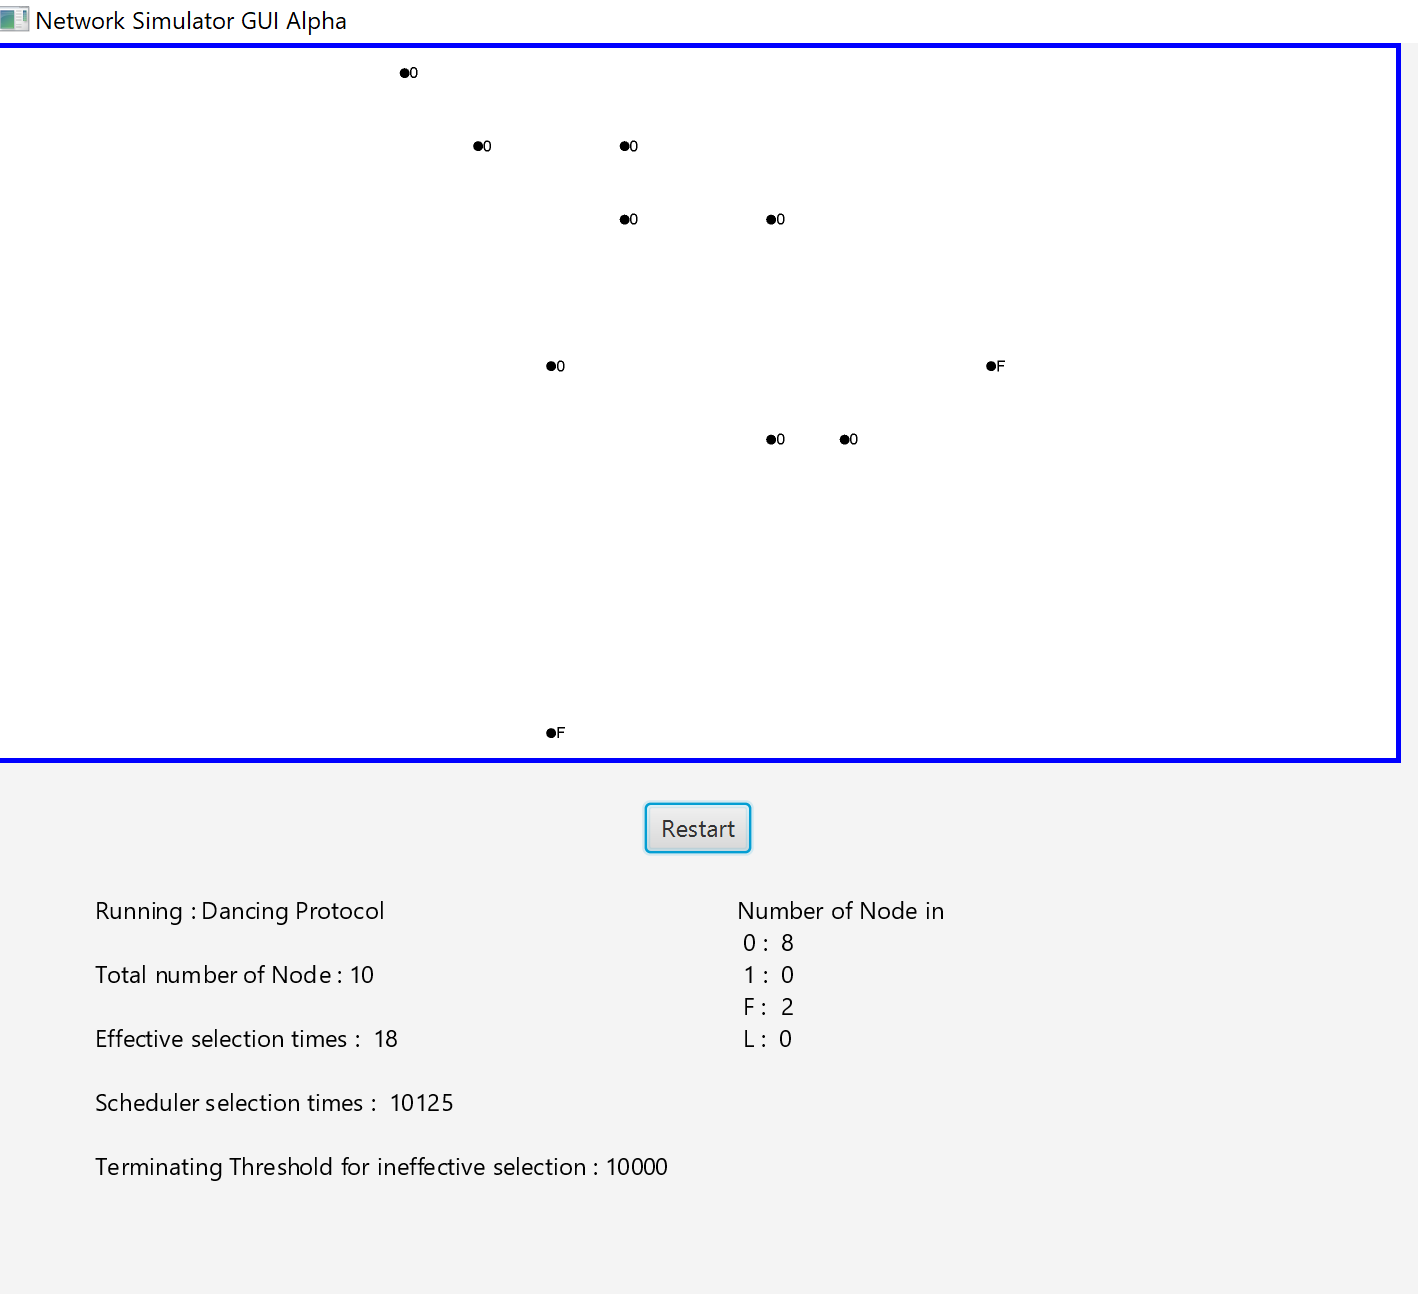
\includegraphics[width =0.45\textwidth]{context/diagram/Dancing_NoneFastForwardingF6.png}
\caption{Result for parameter ID 1 in dancing protocol}
\label{capture_dance_res1}
\end{center}
\end{figure}
\par\noindent
In non-fast-forwarding situation, the scheduler will stop simulation after a consistent ineffective interaction
large than the fixed threshold. In this case, the threshold value is 10000 while the scheduler selects 10125 times in total,
hence it can be concluded that the scheduler selects 10125 - 10000 = 125 times during the simulation process.

\FloatBarrier
\begin{figure}[H]
\begin{center}
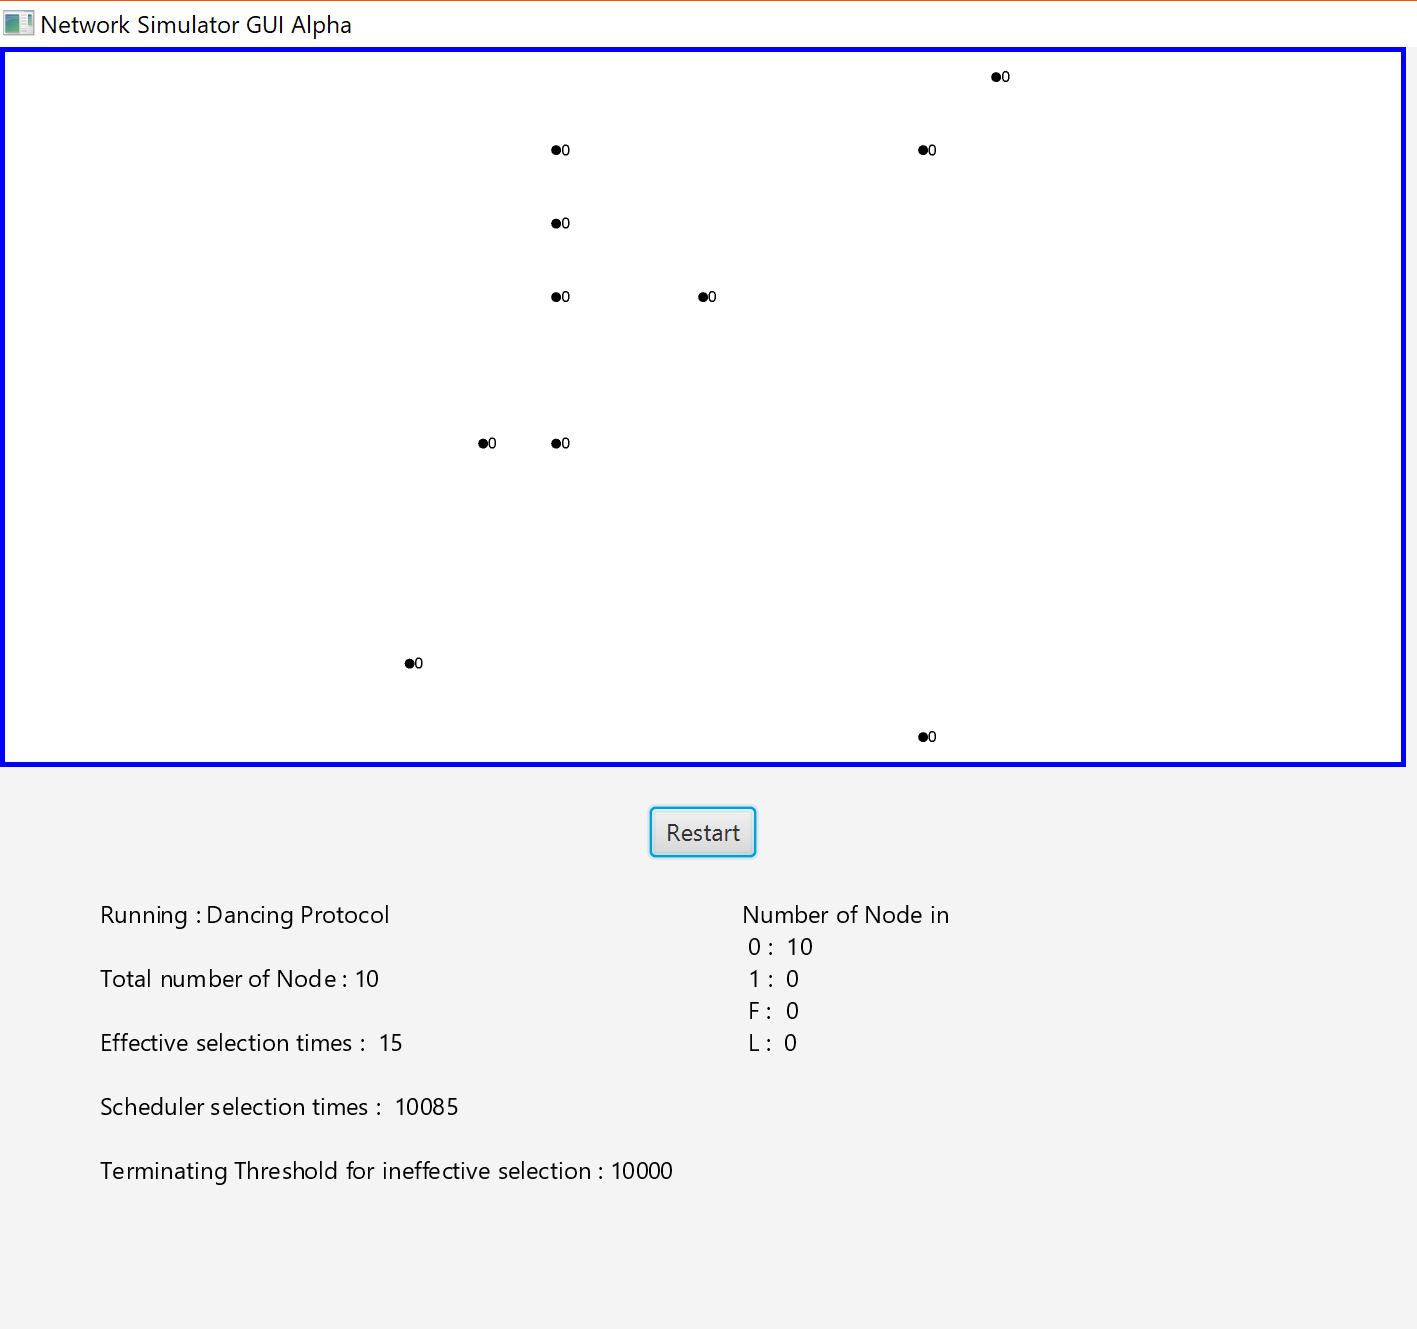
\includegraphics[width =0.45\textwidth]{context/diagram/Dancing_NoneFastForwardingF5.png}
\caption{Result for parameter ID 2 in dancing protocol}
\label{capture_dance_res2}
\end{center}
\end{figure}
\par\noindent
In this case ID 2, the threshold value is 10000 while the scheduler selects 10085 times in total,
hence it can be concluded that the scheduler selects 10085 - 10000 = 85 times during the simulation process.

\FloatBarrier
\begin{figure}[H]
\begin{center}
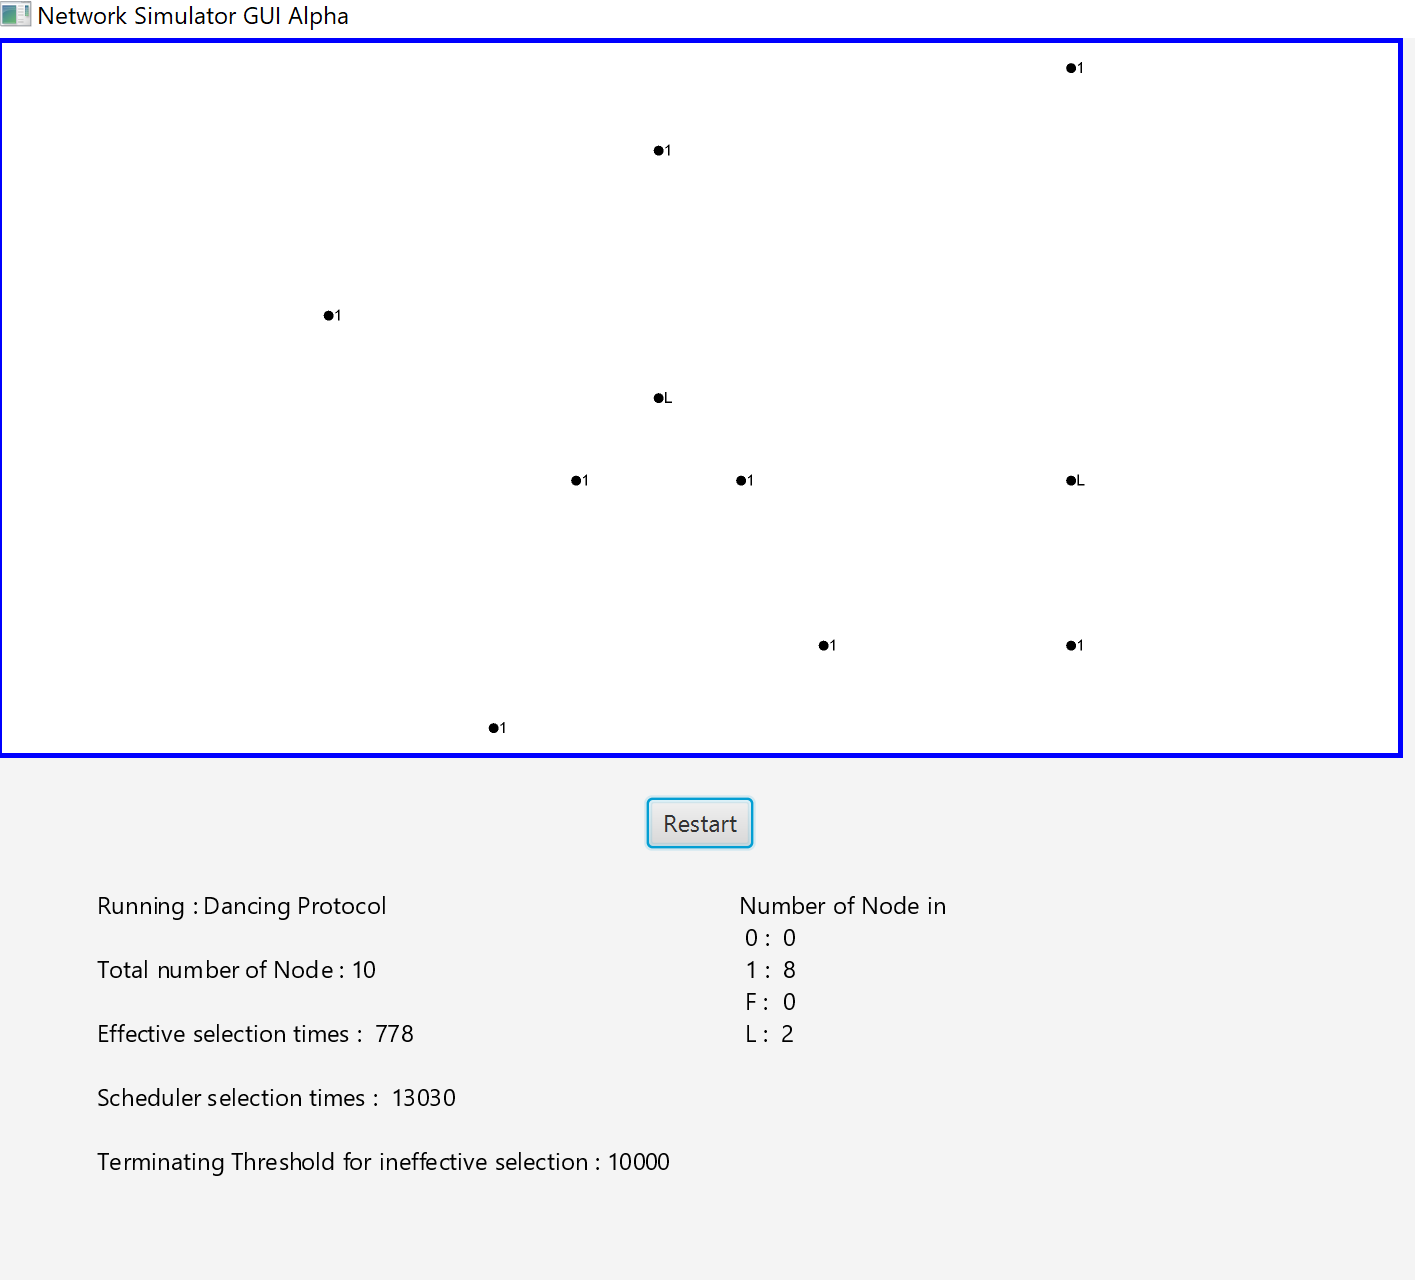
\includegraphics[width =0.45\textwidth]{context/diagram/Dancing_NoneFastForwardingF4.png}
\caption{Result for parameter ID 3 in dancing protocol}
\label{capture_dance_res3}
\end{center}
\end{figure}
\par\noindent
In this case ID 3, the threshold value is 10000 while the scheduler selects 10085 times in total,
hence it can be concluded that the scheduler selects 13030 - 10000 = 3030 times during the simulation process., which is much larger than the previous 2 cases (parameter ID 1 and 2).
From observation of the entire simulation process, the state "F" disappeared in the population at a very early step while
the number of the state "L" also had a stable value 2 from very early beginning .
The state "0" and "1" states were transferred to each other consistently so it is hard to form a convergence.
The set of parameters lead the dancing protocol becoming a protocol that is hard to converge, or say "inefficient".

\subsection{Network Constructor: Experimental simulation for global star protocol}

\FloatBarrier
\begin{table}[H]
\centering
\caption{Experiment parameters for global star protocol}
\label{starParas}
\begin{tabular}{|c|c|c|c|c|}
\hline
ID & \#Nodes & Inital State: c & Enable Fast-forwarding & \#Steps of  Fast-forwarding \\ \hline
1  & 100     & 100             & Yes                    & 1000000                     \\ \hline
2  & 10      & 10              & No                     & Not Applicable              \\ \hline
3  & 50      & 50              & No                     & Not Applicable              \\ \hline
\end{tabular}
\end{table}

\FloatBarrier
\begin{figure}[H]
\begin{center}
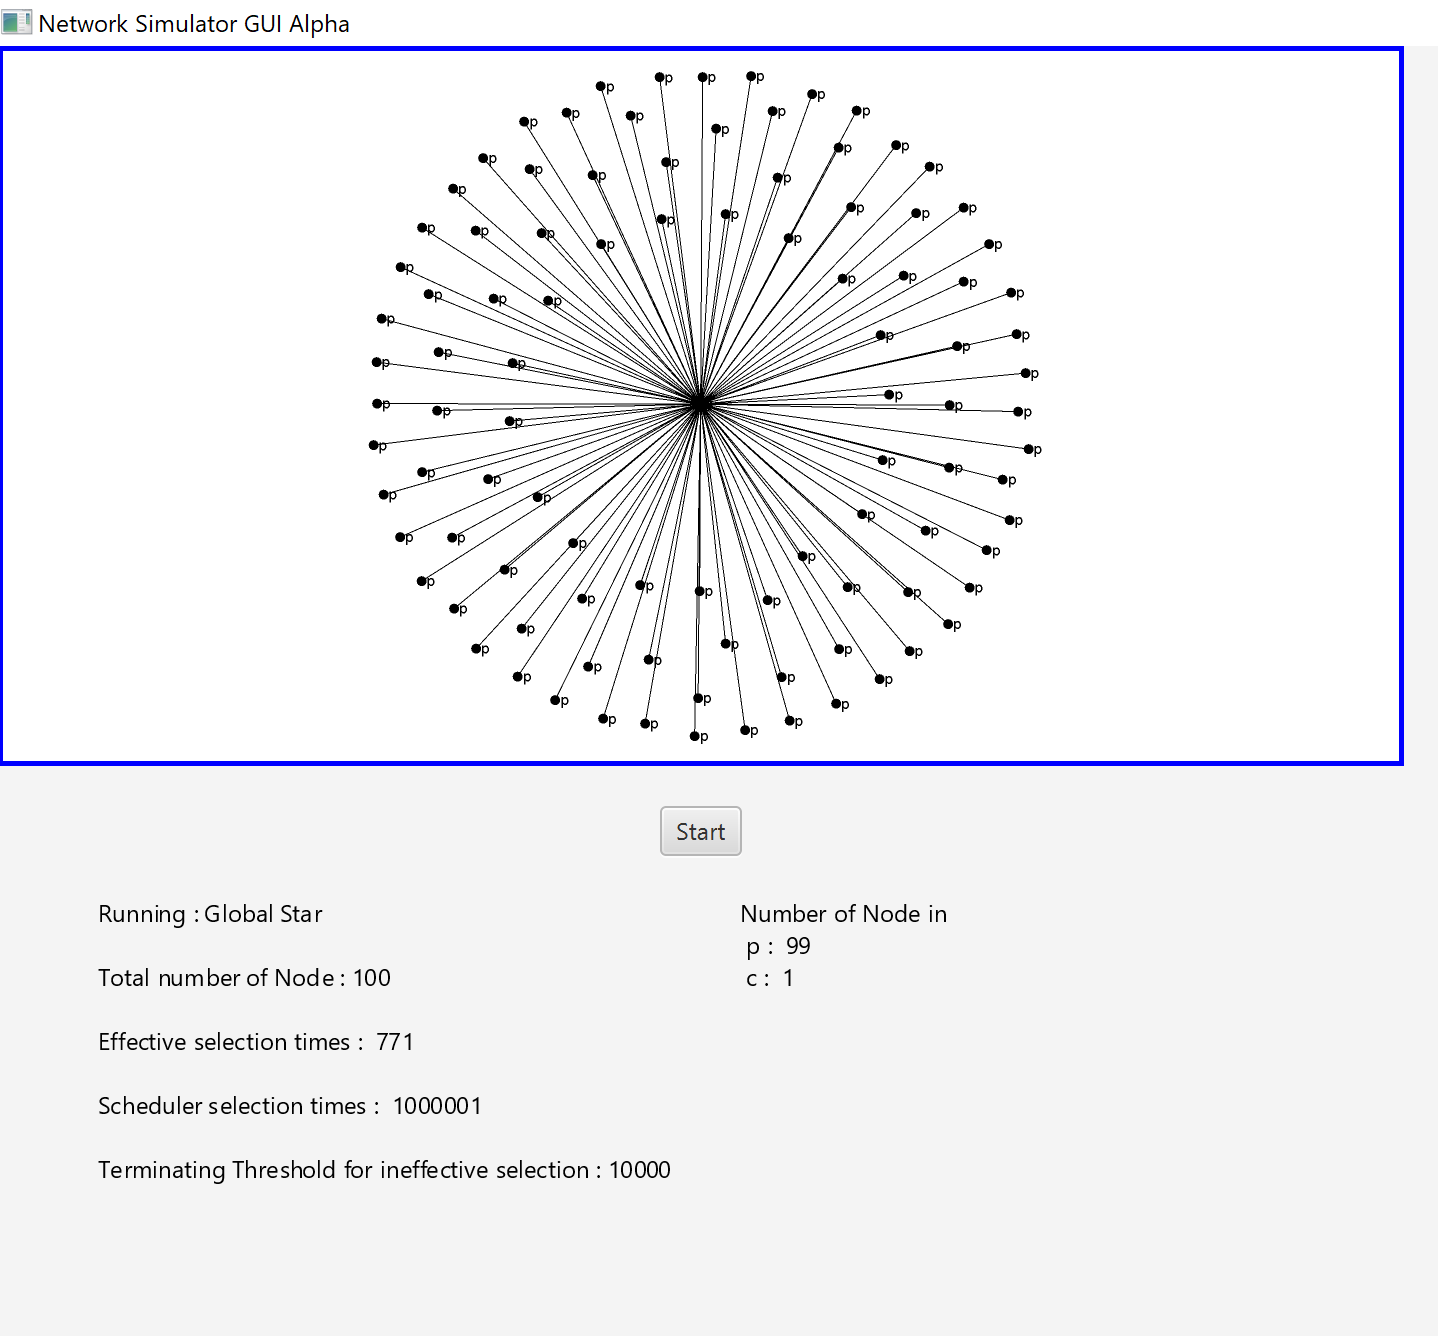
\includegraphics[width =0.45\textwidth]{context/diagram/GlobalStar_FastForwarding_Partial.png}
\caption{Result for parameter ID 1 in global star protocol}
\label{capture_star_res1}
\end{center}
\end{figure}

\par\noindent
In fast-forwarding situation, the scheduler will be forced to executed the given number of selections.
Because the parameter is large enough (1000000), hence it forms the final desired output graph.
This case shows that the simulator is able to simulate the network constructor model.
\FloatBarrier
\begin{figure}[H]
\begin{center}
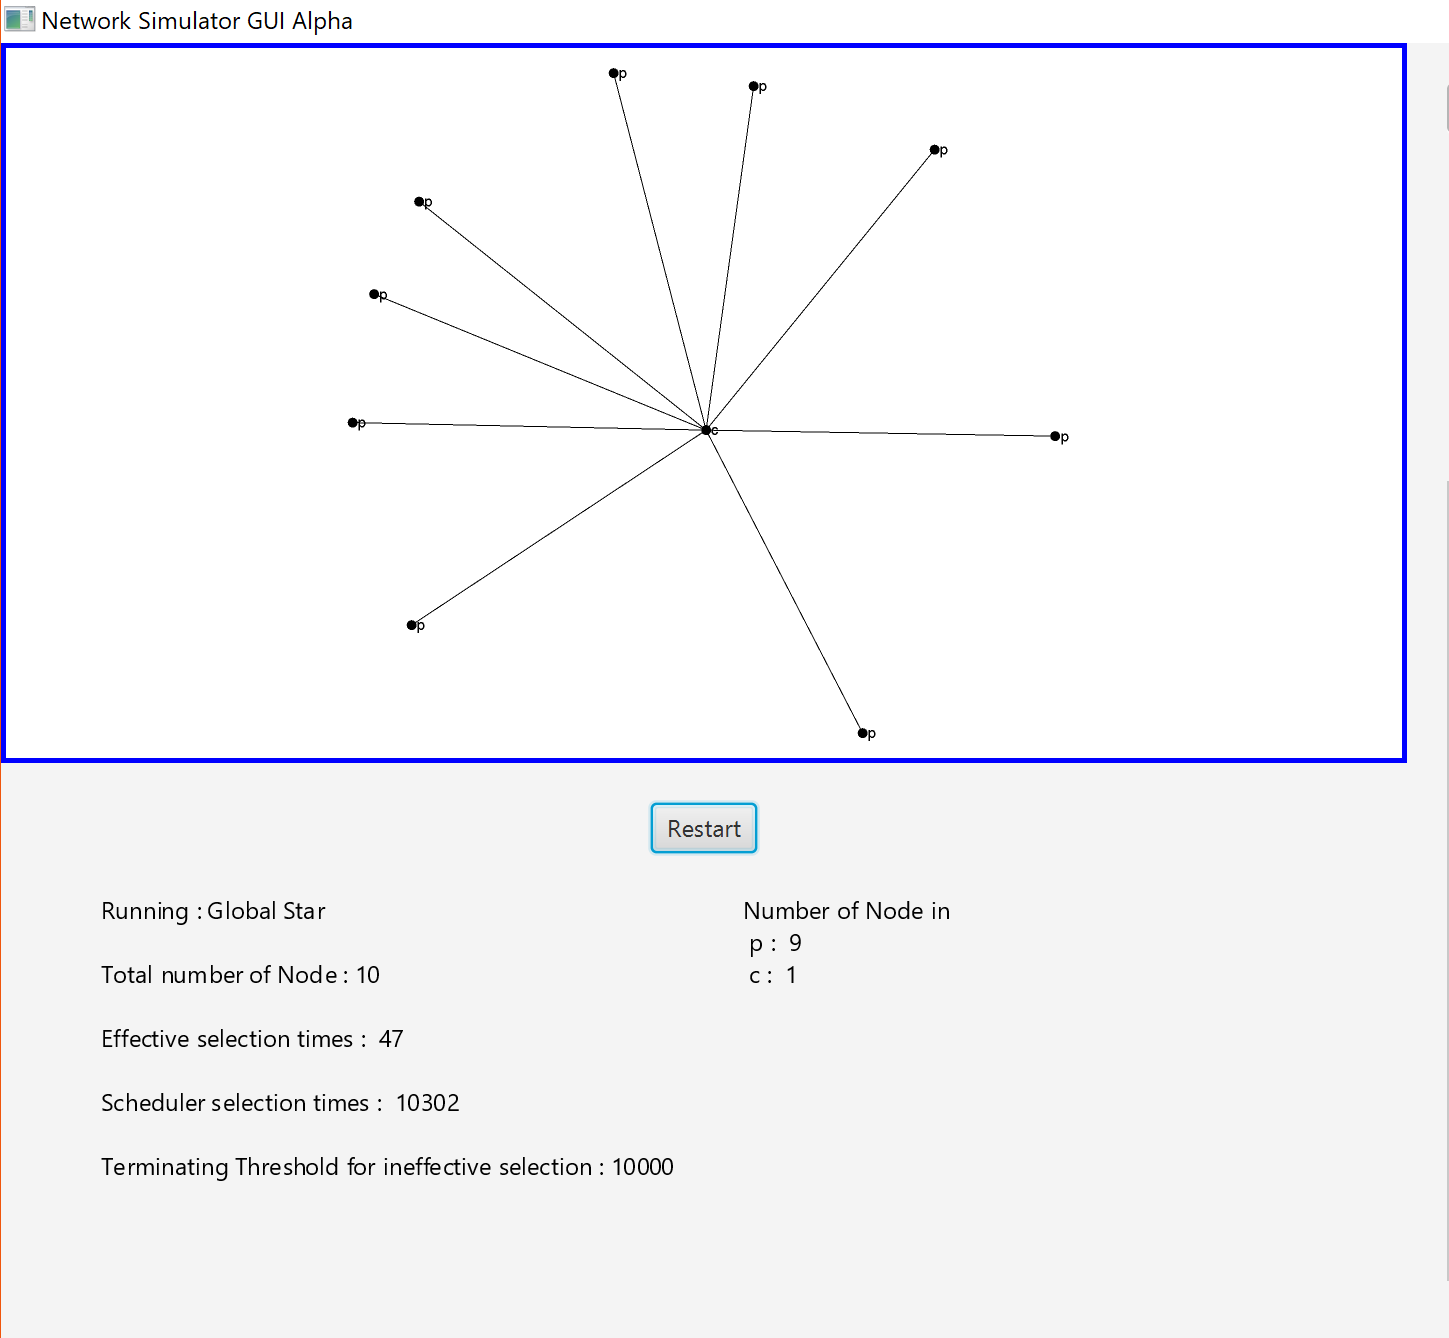
\includegraphics[width =0.45\textwidth]{context/diagram/GlobalStar_NoneFastForwarding10_Partial.png}
\caption{Result for parameter ID 2 in global star protocol}
\label{capture_star_res2}
\end{center}
\end{figure}
\par\noindent
In this case, the threshold value is 10000 while the scheduler selects 10302 times in total,
hence it can be concluded that the scheduler selects 10302 - 10000 = 302 times during the simulation process.
\FloatBarrier
\begin{figure}[H]
\begin{center}
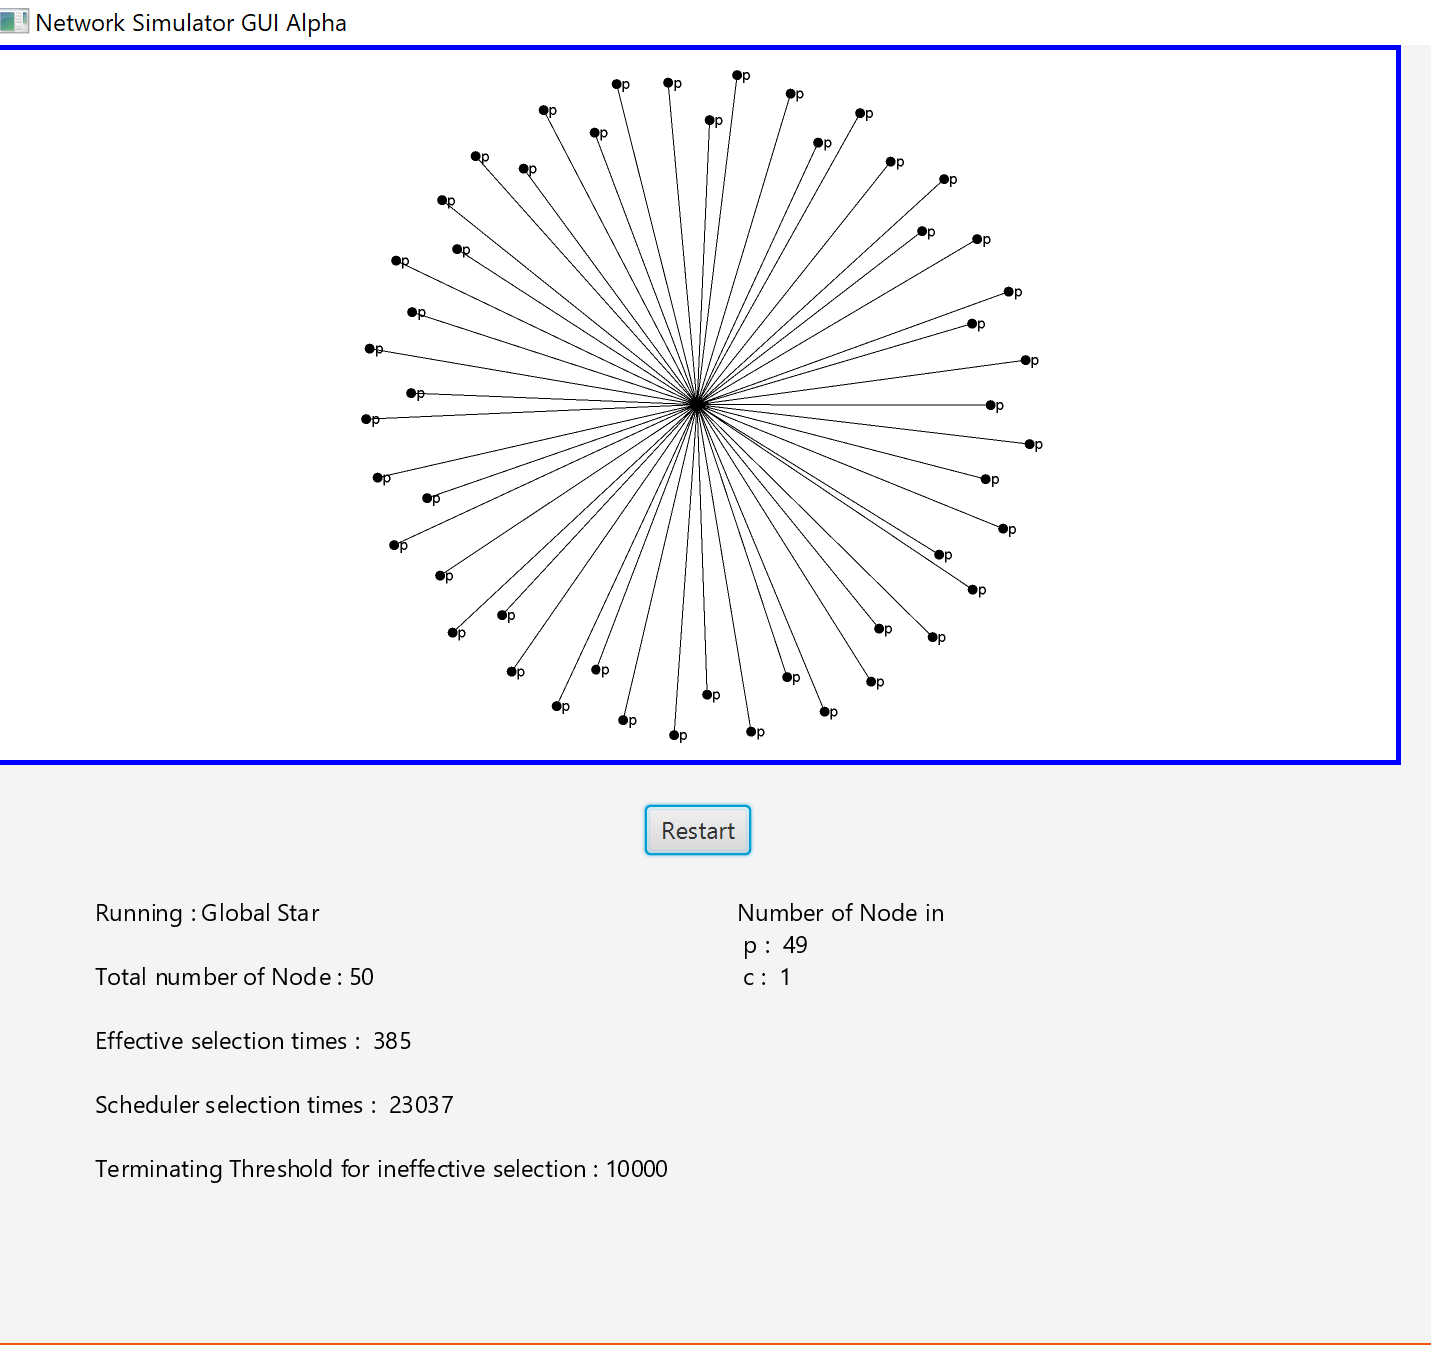
\includegraphics[width =0.45\textwidth]{context/diagram/GlobalStar_NoneFastForwarding50_Partial.png}
\caption{Result for parameter ID 3 in global star protocol}
\label{capture_star_res3}
\end{center}
\end{figure}

\par\noindent
Similar calculation like in parameter ID 2, the scheduler took 23037 - 10000 = 13037 times selection during simulation process.

\par \noindent
Compare parameter ID 2 and 3, it can be noticed the nodes number in ID 3 is 5 times of 10, which is that corresponding number in ID 2.
Nonetheless, the number of scheduler selection in ID 3, 13037, equals to almost 43 times of 302, which is that corresponding value in ID 2.
This may demonstrate that the increase of number of nodes would increases the expected convergence time in a non-linear way for network constructor model.

\subsection{Terminating grid network constructor: Experimental simulation for grid network protocol}
\FloatBarrier
\begin{table}[H]
\centering
\caption{Experiment parameters for grid network protocol}
\label{my-label}
\begin{tabular}{|c|c|c|c|c|}
\hline
ID & \#Nodes & Inital State: $q_{0}$      & Enable Fast-forwarding & \#Steps of  Fast-forwarding \\ \hline
1  & 49      & 48                         & Yes                    & 2000000                     \\ \hline
2  & 9       & 8                          & No                     & Not Applicable              \\ \hline
3  & 25      & 24                         & No                     & Not Applicable              \\ \hline
\end{tabular}
\end{table}

Notice that there is always a node in state "$L_{u}$" at initial for grid network protocol.
\FloatBarrier
\begin{figure}[H]
\begin{center}
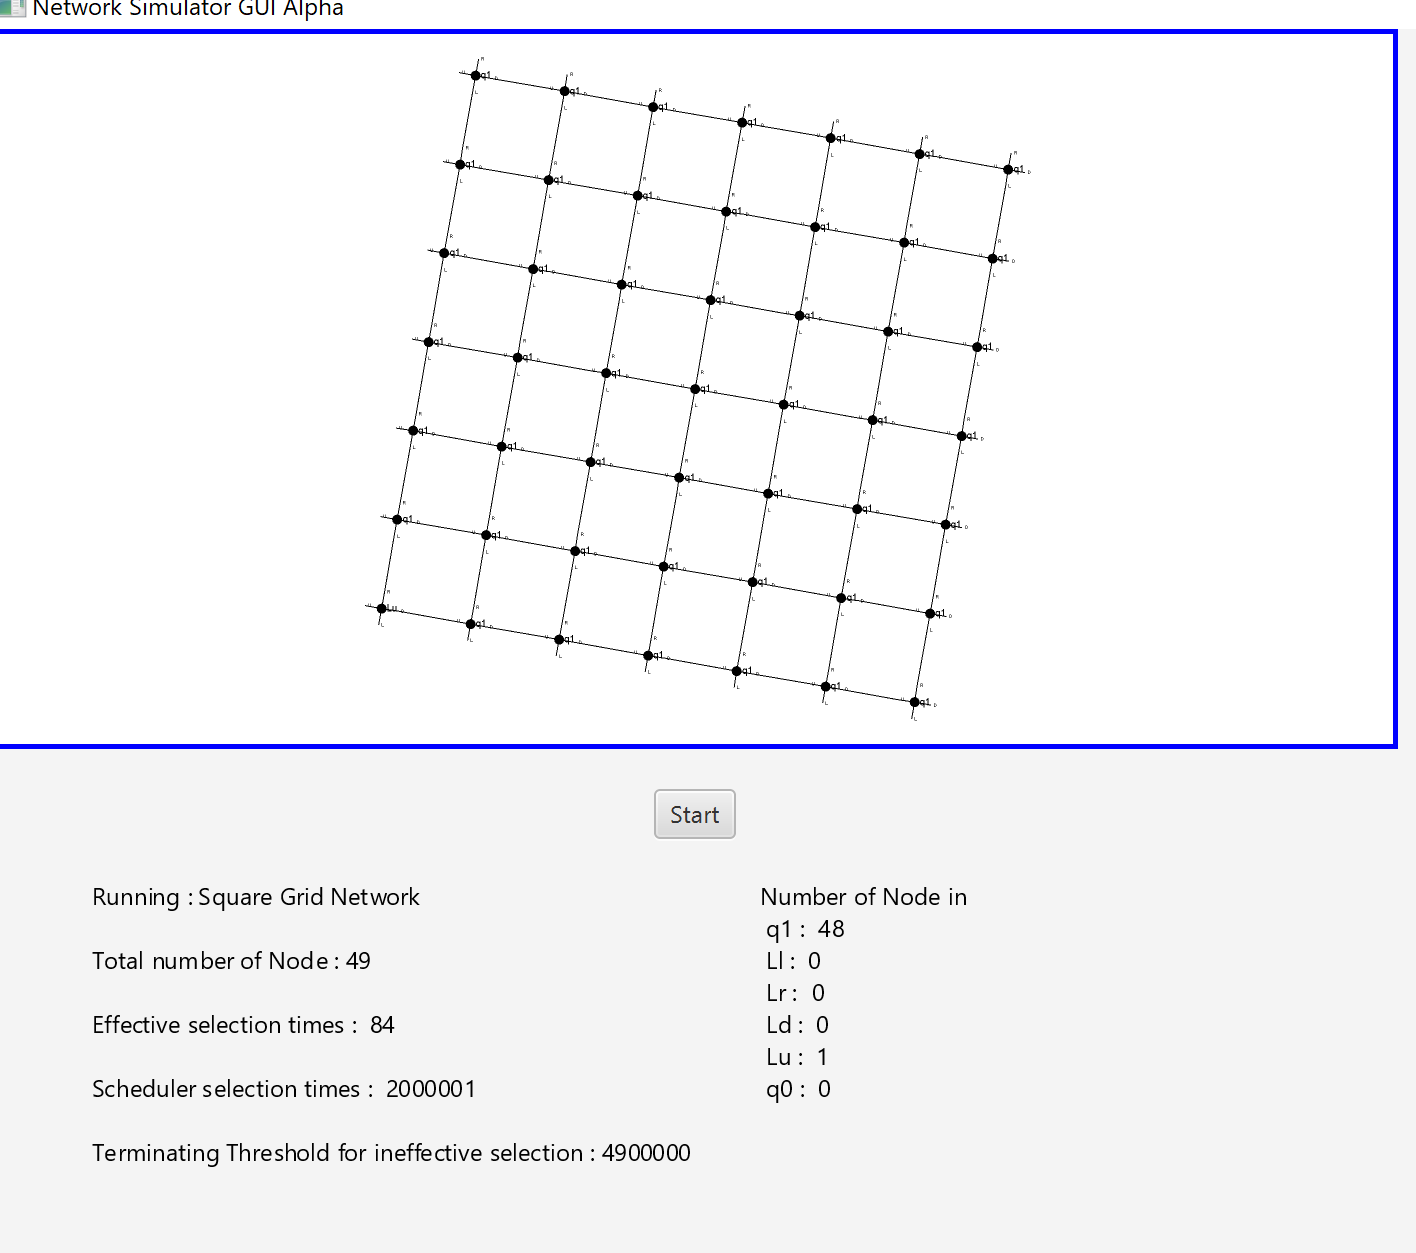
\includegraphics[width =0.45\textwidth]{context/diagram/GridNetwork_FastForwarding_Partial.png}
\caption{Result for parameter ID 1 in grid network protocol}
\label{capture_grid_res1}
\end{center}
\end{figure}
\par\noindent
Again it is in fast-forwarding model and because the parameter is large enough (2000000), it forms the final desired output graph.
This case shows that the simulator is able to simulate the terminating grid network constructor model.
\FloatBarrier
\begin{figure}[H]
\begin{center}
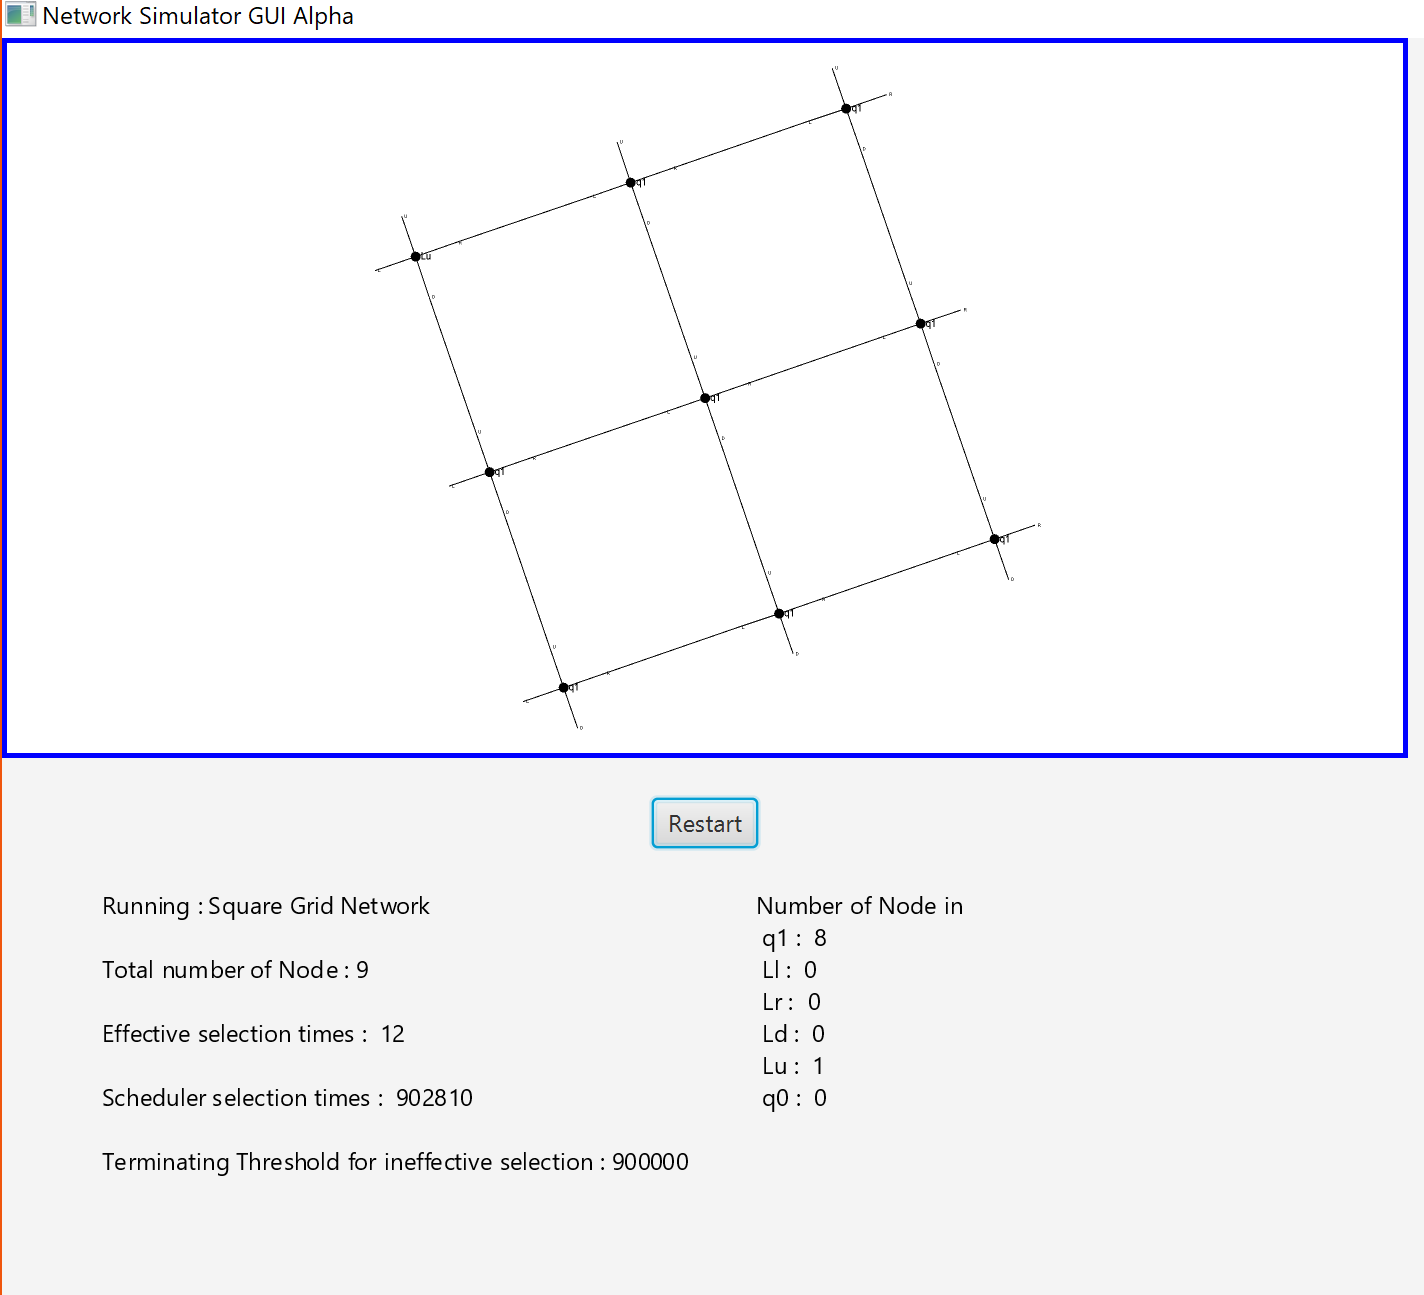
\includegraphics[width =0.45\textwidth]{context/diagram/GridNetwork_NoneFastForwarding8_Partial.png}
\caption{Result for parameter ID 2 in grid network protocol}
\label{capture_grid_res2}
\end{center}
\end{figure}
\par\noindent
It is in none-fast-forwarding model, hence it can be concluded that the scheduler selects 902810 - 900000 = 2810 times during the simulation process.
\FloatBarrier
\begin{figure}[H]
\begin{center}
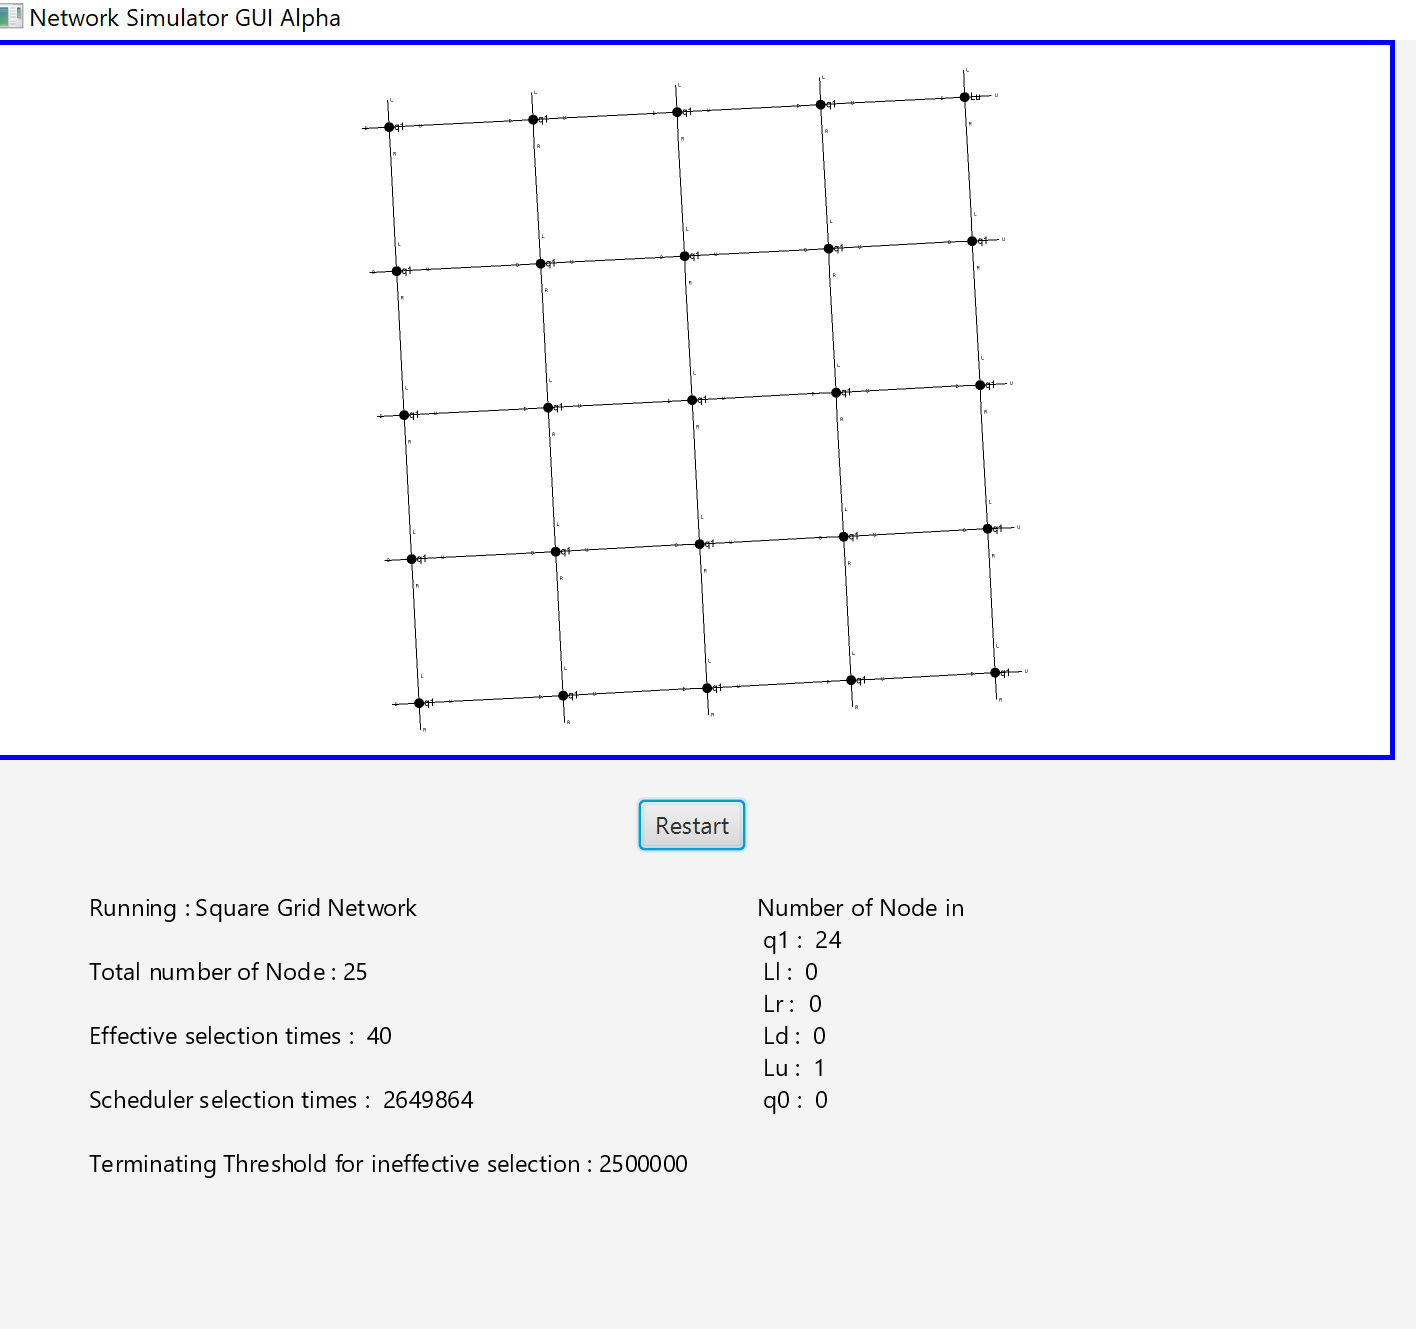
\includegraphics[width =0.45\textwidth]{context/diagram/GridNetwork_NoneFastForwarding24_Partial.png}
\caption{Result for parameter ID 3 in grid network protocol}
\label{capture_grid_res3}
\end{center}
\end{figure}
\par\noindent
Again it is in none-fast-forwarding model, hence it can be concluded that the scheduler selects 2649864 - 2500000 = 149864 times during the simulation process.
Compared with results in parameter ID 2 and parameter ID 3, it might be concluded that the increase of number of nodes would increases the expected termination time in a non-linear way for terminating grid network constructor model.

\subsection{Critical evaluation}
The project is generally successful. The simulator finishes most functionality and was proved that it can simulate all three kinds of population,
hence it enabled the author to start some simple experiments and it can be concluded that increasing of the
number of nodes will increase the expected convergence or termination time for network constructor and terminating grid network constructor.
For dancing protocol, a set of initial setting that may lead to hard to converge is also identified.
Generally, the two criteria mentioned in previous section are satisfied though there is also some flaws existing in the implementation, for example,
the user interface cannot to be resized due to some technical issues (because two incompatible user interface software library mixed).

\subsection{Strength and weakness of the project}
\par\noindent
\paragraph{Strength}
\begin{itemize}
  \item The most requirements are successfully finished.
  \item The simulator is easy to extend in terms of protocols.
  \item The project may help studies and researches with regards to population protocols.
  \item The experiment does reveals the inefficiency (or hardness to converge) for dancing protocol under the initial settings that the number of leaders is slightly larger than that of the followers in the population.
\end{itemize}
\paragraph{Weakness and points to further improvement}
\begin{itemize}
  \item The axisymmetric cases for eliminating overlap has not been implemented in grid terminating network constructor,
  this may requires further development.
  \item The simulator cannot be resizable. It should be resolved latter on via moving Java Swing to JavaFX later on.
  \item If possible, it still should provide an simple interface (or DSL) to allow the users to directly write some protocol definitions in a more simple way.
\end{itemize}
